\section{Sets and Relations}

\begin{definition}[Polyhedral Set]
A {\em polyhedral set}\index{polyhedral set} $S$ is a finite union of basic sets
$S = \bigcup_i S_i$, each of which can be represented using affine
constraints
$$
S_i : \Z^n \to 2^{\Z^d} : \vec s \mapsto
S_i(\vec s) =
\{\, \vec x \in \Z^d \mid \exists \vec z \in \Z^e :
A \vec x + B \vec s + D \vec z + \vec c \geq \vec 0 \,\}
,
$$
with $A \in \Z^{m \times d}$,
$B \in \Z^{m \times n}$,
$D \in \Z^{m \times e}$
and $\vec c \in \Z^m$.
\end{definition}

\begin{definition}[Parameter Domain of a Set]
Let $S \in \Z^n \to 2^{\Z^d}$ be a set.
The {\em parameter domain} of $S$ is the set
$$\pdom S \coloneqq \{\, \vec s \in \Z^n \mid S(\vec s) \ne \emptyset \,\}.$$
\end{definition}

\begin{definition}[Polyhedral Relation]
A {\em polyhedral relation}\index{polyhedral relation}
$R$ is a finite union of basic relations
$R = \bigcup_i R_i$ of type
$\Z^n \to 2^{\Z^{d_1+d_2}}$,
each of which can be represented using affine
constraints
$$
R_i = \vec s \mapsto
R_i(\vec s) =
\{\, \vec x_1 \to \vec x_2 \in \Z^{d_1} \times \Z^{d_2}
\mid \exists \vec z \in \Z^e :
A_1 \vec x_1 + A_2 \vec x_2 + B \vec s + D \vec z + \vec c \geq \vec 0 \,\}
,
$$
with $A_i \in \Z^{m \times d_i}$,
$B \in \Z^{m \times n}$,
$D \in \Z^{m \times e}$
and $\vec c \in \Z^m$.
\end{definition}

\begin{definition}[Parameter Domain of a Relation]
Let $R \in \Z^n \to 2^{\Z^{d+d}}$ be a relation.
The {\em parameter domain} of $R$ is the set
$$\pdom R \coloneqq \{\, \vec s \in \Z^n \mid R(\vec s) \ne \emptyset \,\}.$$
\end{definition}

\begin{definition}[Domain of a Relation]
Let $R \in \Z^n \to 2^{\Z^{d+d}}$ be a relation.
The {\em domain} of $R$ is the polyhedral set
$$\domain R \coloneqq \vec s \mapsto
\{\, \vec x_1 \in \Z^{d_1} \mid \exists \vec x_2 \in \Z^{d_2} :
(\vec x_1, \vec x_2) \in R(\vec s) \,\}
.
$$
\end{definition}

\begin{definition}[Range of a Relation]
Let $R \in \Z^n \to 2^{\Z^{d+d}}$ be a relation.
The {\em range} of $R$ is the polyhedral set
$$
\range R \coloneqq \vec s \mapsto
\{\, \vec x_2 \in \Z^{d_2} \mid \exists \vec x_1 \in \Z^{d_1} :
(\vec x_1, \vec x_2) \in R(\vec s) \,\}
.
$$
\end{definition}

\begin{definition}[Composition of Relations]
Let $R \in \Z^n \to 2^{\Z^{d_1+d_2}}$ and
$S \in \Z^n \to 2^{\Z^{d_2+d_3}}$ be two relations,
then the composition of
$R$ and $S$ is defined as
$$
S \circ R \coloneqq
\vec s \mapsto
\{\, \vec x_1 \to \vec x_3 \in \Z^{d_1} \times \Z^{d_3}
\mid \exists \vec x_2 \in \Z^{d_2} :
\vec x_1 \to \vec x_2 \in R(\vec s) \wedge
\vec x_2 \to \vec x_3 \in S(\vec s)
\,\}
.
$$
\end{definition}

\begin{definition}[Difference Set of a Relation]
Let $R \in \Z^n \to 2^{\Z^{d+d}}$ be a relation.
The difference set ($\Delta \, R$) of $R$ is the set
of differences between image elements and the corresponding
domain elements,
$$
\Delta \, R \coloneqq
\vec s \mapsto
\{\, \vec \delta \in \Z^{d} \mid \exists \vec x \to \vec y \in R :
\vec \delta = \vec y - \vec x
\,\}
$$
\end{definition}

\section{Coalescing}\label{s:coalescing}

See \shortciteN{Verdoolaege2009isl}, for now.
More details will be added later.

\section{Transitive Closure}

\subsection{Introduction}

\begin{definition}[Power of a Relation]
Let $R \in \Z^n \to 2^{\Z^{d+d}}$ be a relation and
$k \in \Z_{\ge 1}$
a positive number, then power $k$ of relation $R$ is defined as
\begin{equation}
\label{eq:transitive:power}
R^k \coloneqq
\begin{cases}
R & \text{if $k = 1$}
\\
R \circ R^{k-1} & \text{if $k \ge 2$}
.
\end{cases}
\end{equation}
\end{definition}

\begin{definition}[Transitive Closure of a Relation]
Let $R \in \Z^n \to 2^{\Z^{d+d}}$ be a relation,
then the transitive closure $R^+$ of $R$ is the union
of all positive powers of $R$,
$$
R^+ \coloneqq \bigcup_{k \ge 1} R^k
.
$$
\end{definition}
Alternatively, the transitive closure may be defined
inductively as
\begin{equation}
\label{eq:transitive:inductive}
R^+ \coloneqq R \cup \left(R \circ R^+\right)
.
\end{equation}

Since the transitive closure of a polyhedral relation
may no longer be a polyhedral relation \shortcite{Kelly1996closure},
we can, in the general case, only compute an approximation
of the transitive closure.
Whereas \shortciteN{Kelly1996closure} compute underapproximations,
we, like \shortciteN{Beletska2009}, compute overapproximations.
That is, given a relation $R$, we will compute a relation $T$
such that $R^+ \subseteq T$.  Of course, we want this approximation
to be as close as possible to the actual transitive closure
$R^+$ and we want to detect the cases where the approximation is
exact, i.e., where $T = R^+$.

For computing an approximation of the transitive closure of $R$,
we follow the same general strategy as \shortciteN{Beletska2009}
and first compute an approximation of $R^k$ for $k \ge 1$ and then project
out the parameter $k$ from the resulting relation.

\begin{example}
As a trivial example, consider the relation
$R = \{\, x \to x + 1 \,\}$.  The $k$th power of this map
for arbitrary $k$ is
$$
R^k = k \mapsto \{\, x \to x + k \mid k \ge 1 \,\}
.
$$
The transitive closure is then
$$
\begin{aligned}
R^+ & = \{\, x \to y \mid \exists k \in \Z_{\ge 1} : y = x + k \,\}
\\
& = \{\, x \to y \mid y \ge x + 1 \,\}
.
\end{aligned}
$$
\end{example}

\subsection{Computing an Approximation of $R^k$}
\label{s:power}

There are some special cases where the computation of $R^k$ is very easy.
One such case is that where $R$ does not compose with itself,
i.e., $R \circ R = \emptyset$ or $\domain R \cap \range R = \emptyset$.
In this case, $R^k$ is only non-empty for $k=1$ where it is equal
to $R$ itself.

In general, it is impossible to construct a closed form
of $R^k$ as a polyhedral relation.
We will therefore need to make some approximations.
As a first approximations, we will consider each of the basic
relations in $R$ as simply adding one or more offsets to a domain element
to arrive at an image element and ignore the fact that some of these
offsets may only be applied to some of the domain elements.
That is, we will only consider the difference set $\Delta\,R$ of the relation.
In particular, we will first construct a collection $P$ of paths
that move through
a total of $k$ offsets and then intersect domain and range of this
collection with those of $R$.
That is, 
\begin{equation}
\label{eq:transitive:approx}
K = P \cap \left(\domain R \to \range R\right)
,
\end{equation}
with
\begin{equation}
\label{eq:transitive:path}
P = \vec s \mapsto \{\, \vec x \to \vec y \mid
\exists k_i \in \Z_{\ge 0} :
\vec y = \vec x + \sum_i k_i \, \Delta_i(\vec s)
\wedge
\sum_i k_i = k > 0
\,\}
\end{equation}
and with $\Delta_i$ the basic sets that compose
the difference set $\Delta\,R$.
Note that the number of basic sets $\Delta_i$ need not be
the same as the number of basic relations in $R$.
Also note that since addition is commutative, it does not
matter in which order we add the offsets and so we are allowed
to group them as we did in \eqref{eq:transitive:path}.

If all the $\Delta_i$s are singleton sets
$\Delta_i = \{\, \vec \delta_i \,\}$ with $\vec \delta_i \in \Z^d$,
then \eqref{eq:transitive:path} simplifies to
\begin{equation}
\label{eq:transitive:singleton}
P = \{\, \vec x \to \vec y \mid
\exists k_i \in \Z_{\ge 0} :
\vec y = \vec x + \sum_i k_i \, \vec \delta_i
\wedge
\sum_i k_i = k > 0
\,\}
\end{equation}
and then the approximation computed in \eqref{eq:transitive:approx}
is essentially the same as that of \shortciteN{Beletska2009}.
If some of $\Delta_i$s are not singleton sets or if
some of $\vec \delta_i$s are parametric, then we need
to resort to further approximations.

To ease both the exposition and the implementation, we will for
the remainder of this section work with extended offsets
$\Delta_i' = \Delta_i \times \{\, 1 \,\}$.
That is, each offset is extended with an extra coordinate that is
set equal to one.  The paths constructed by summing such extended
offsets have the length encoded as the difference of their
final coordinates.  The path $P'$ can then be decomposed into
paths $P_i'$, one for each $\Delta_i$,
\begin{equation}
\label{eq:transitive:decompose}
P' = \left(
(P_m' \cup \identity) \circ \cdots \circ
(P_2' \cup \identity) \circ
(P_1' \cup \identity)
\right) \cap
\{\,
\vec x' \to \vec y' \mid y_{d+1} - x_{d+1} = k > 0
\,\}
,
\end{equation}
with
$$
P_i' = \vec s \mapsto \{\, \vec x' \to \vec y' \mid
\exists k \in \Z_{\ge 1} :
\vec y' = \vec x' + k \, \Delta_i'(\vec s)
\,\}
.
$$
Note that each $P_i'$ contains paths of length at least one.
We therefore need to take the union with the identity relation
when composing the $P_i'$s to allow for paths that do not contain
any offsets from one or more $\Delta_i'$.
The path that consists of only identity relations is removed
by imposing the constraint $y_{d+1} - x_{d+1} > 0$.
Taking the union with the identity relation means that
that the relations we compose in \eqref{eq:transitive:decompose}
each consist of two basic relations.  If there are $m$
disjuncts in the input relation, then a direct application
of the composition operation may therefore result in a relation
with $2^m$ disjuncts, which is prohibitively expensive.
It is therefore crucial to apply coalescing (\autoref{s:coalescing})
after each composition.

Let us now consider how to compute an overapproximation of $P_i'$.
Those that correspond to singleton $\Delta_i$s are grouped together
and handled as in \eqref{eq:transitive:singleton}.
Note that this is just an optimization.  The procedure described
below would produce results that are at least as accurate.
For simplicity, we first assume that no constraint in $\Delta_i'$
involves any existentially quantified variables.
We will return to existentially quantified variables at the end
of this section.
Without existentially quantified variables, we can classify
the constraints of $\Delta_i'$ as follows
\begin{enumerate}
\item non-parametric constraints
\begin{equation}
\label{eq:transitive:non-parametric}
A_1 \vec x + \vec c_1 \geq \vec 0
\end{equation}
\item purely parametric constraints
\begin{equation}
\label{eq:transitive:parametric}
B_2 \vec s + \vec c_2 \geq \vec 0
\end{equation}
\item negative mixed constraints
\begin{equation}
\label{eq:transitive:mixed}
A_3 \vec x + B_3 \vec s + \vec c_3 \geq \vec 0
\end{equation}
such that for each row $j$ and for all $\vec s$,
$$
\Delta_i'(\vec s) \cap
\{\, \vec x' \to \vec y' \mid B_{3,j} \vec s + c_{3,j} > 0 \,\}
= \emptyset
$$
\item positive mixed constraints
$$
A_4 \vec x + B_4 \vec s + \vec c_4 \geq \vec 0
$$
such that for each row $j$, there is at least one $\vec s$ such that
$$
\Delta_i'(\vec s) \cap
\{\, \vec x' \to \vec y' \mid B_{4,j} \vec s + c_{4,j} > 0 \,\}
\ne \emptyset
$$
\end{enumerate}
We will use the following approximation $Q_i$ for $P_i'$:
\begin{equation}
\label{eq:transitive:Q}
\begin{aligned}
Q_i = \vec s \mapsto
\{\,
\vec x' \to \vec y'
\mid {} & \exists k \in \Z_{\ge 1}, \vec f \in \Z^d :
\vec y' = \vec x' + (\vec f, k)
\wedge {}
\\
&
A_1 \vec f + k \vec c_1 \geq \vec 0
\wedge
B_2 \vec s + \vec c_2 \geq \vec 0
\wedge
A_3 \vec f + B_3 \vec s + \vec c_3 \geq \vec 0
\,\}
.
\end{aligned}
\end{equation}
To prove that $Q_i$ is indeed an overapproximation of $P_i'$,
we need to show that for every $\vec s \in \Z^n$, for every
$k \in \Z_{\ge 1}$ and for every $\vec f \in k \, \Delta_i(\vec s)$
we have that
$(\vec f, k)$ satisfies the constraints in \eqref{eq:transitive:Q}.
If $\Delta_i(\vec s)$ is non-empty, then $\vec s$ must satisfy
the constraints in \eqref{eq:transitive:parametric}.
Each element $(\vec f, k) \in k \, \Delta_i'(\vec s)$ is a sum
of $k$ elements $(\vec f_j, 1)$ in $\Delta_i'(\vec s)$.
Each of these elements satisfies the constraints in
\eqref{eq:transitive:non-parametric}, i.e.,
$$
\left[
\begin{matrix}
A_1 & \vec c_1
\end{matrix}
\right]
\left[
\begin{matrix}
\vec f_j \\ 1
\end{matrix}
\right]
\ge \vec 0
.
$$
The sum of these elements therefore satisfies the same set of inequalities,
i.e., $A_1 \vec f + k \vec c_1 \geq \vec 0$.
Finally, the constraints in \eqref{eq:transitive:mixed} are such
that for any $\vec s$ in the parameter domain of $\Delta$,
we have $-\vec r(\vec s) \coloneqq B_3 \vec s + \vec c_3 \le \vec 0$,
i.e., $A_3 \vec f_j \ge \vec r(\vec s) \ge \vec 0$
and therefore also $A_3 \vec f \ge \vec r(\vec s)$.
Note that if there are no mixed constraints and if the
rational relaxation of $\Delta_i(\vec s)$, i.e.,
$\{\, \vec x \in \Q^d \mid A_1 \vec x + \vec c_1 \ge \vec 0\,\}$,
has integer vertices, then the approximation is exact, i.e.,
$Q_i = P_i'$.  In this case, the vertices of $\Delta'_i(\vec s)$
generate the rational cone
$\{\, \vec x' \in \Q^{d+1} \mid \left[
\begin{matrix}
A_1 & \vec c_1
\end{matrix}
\right] \vec x' \,\}$ and therefore $\Delta'_i(\vec s)$ is
a Hilbert basis of this cone \shortcite[Theorem~16.4]{Schrijver1986}.

Existentially quantified variables can be handled by
classifying them into variables that are uniquely
determined by the parameters, variables that are independent
of the parameters and others.  The first set can be treated
as parameters and the second as variables.  Constraints involving
the other existentially quantified variables are removed.

\begin{example}
Consider the relation
$$
R =
n \to \{\, x \to y \mid \exists \, \alpha_0, \alpha_1: 7\alpha_0 = -2 + n \wedge 5\alpha_1 = -1 - x + y \wedge y \ge 6 + x \,\}
.
$$
The difference set of this relation is
$$
\Delta = \Delta \, R =
n \to \{\, x \mid \exists \, \alpha_0, \alpha_1: 7\alpha_0 = -2 + n \wedge 5\alpha_1 = -1 + x \wedge x \ge 6 \,\}
.
$$
The existentially quantified variables can be defined in terms
of the parameters and variables as
$$
\alpha_0 = \floor{\frac{-2 + n}7}
\qquad
\text{and}
\qquad
\alpha_1 = \floor{\frac{-1 + x}5}
.
$$
$\alpha_0$ can therefore be treated as a parameter,
while $\alpha_1$ can be treated as a variable.
This in turn means that $7\alpha_0 = -2 + n$ can be treated as
a purely parametric constraint, while the other two constraints are
non-parametric.
The corresponding $Q$~\eqref{eq:transitive:Q} is therefore
$$
\begin{aligned}
n \to \{\, (x,z) \to (y,w) \mid
\exists\, \alpha_0, \alpha_1, k, f : {} &
k \ge 1 \wedge
y = x + f \wedge
w = z + k \wedge {} \\
&
7\alpha_0 = -2 + n \wedge
5\alpha_1 = -k + x \wedge
x \ge 6 k
\,\}
.
\end{aligned}
$$
Projecting out the final coordinates encoding the length of the paths,
results in the exact transitive closure
$$
R^+ =
n \to \{\, x \to y \mid \exists \, \alpha_0, \alpha_1: 7\alpha_1 = -2 + n \wedge 6\alpha_0 \ge -x + y \wedge 5\alpha_0 \le -1 - x + y \,\}
.
$$
\end{example}

\subsection{Checking Exactness}

The approximation $T$ for the transitive closure $R^+$ can be obtained
by projecting out the parameter $k$ from the approximation $K$
\eqref{eq:transitive:approx} of the power $R^k$.
Since $K$ is an overapproximation of $R^k$, $T$ will also be an
overapproximation of $R^+$.
To check whether the results are exact, we need to consider two
cases depending on whether $R$ is {\em cyclic}, where $R$ is defined
to be cyclic if $R^+$ maps any element to itself, i.e.,
$R^+ \cap \identity \ne \emptyset$.
If $R$ is acyclic, then the inductive definition of
\eqref{eq:transitive:inductive} is equivalent to its completion,
i.e.,
$$
R^+ = R \cup \left(R \circ R^+\right)
$$
is a defining property.
Since $T$ is known to be an overapproximation, we only need to check
whether
$$
T \subseteq R \cup \left(R \circ T\right)
.
$$
This is essentially Theorem~5 of \shortciteN{Kelly1996closure}.
The only difference is that they only consider lexicographically
forward relations, a special case of acyclic relations.

If, on the other hand, $R$ is cyclic, then we have to resort
to checking whether the approximation $K$ of the power is exact.
Note that $T$ may be exact even if $K$ is not exact, so the check
is sound, but incomplete.
To check exactness of the power, we simply need to check
\eqref{eq:transitive:power}.  Since again $K$ is known
to be an overapproximation, we only need to check whether
$$
\begin{aligned}
K'|_{y_{d+1} - x_{d+1} = 1} & \subseteq R'
\\
K'|_{y_{d+1} - x_{d+1} \ge 2} & \subseteq R' \circ K'|_{y_{d+1} - x_{d+1} \ge 1}
,
\end{aligned}
$$
where $R' = \{\, \vec x' \to \vec y' \mid \vec x \to \vec y \in R
\wedge y_{d+1} - x_{d+1} = 1\,\}$, i.e., $R$ extended with path
lengths equal to 1.

All that remains is to explain how to check the cyclicity of $R$.
Note that the exactness on the power is always sound, even
in the acyclic case, so we only need to be careful that we find
all cyclic cases.  Now, if $R$ is cyclic, i.e.,
$R^+ \cap \identity \ne \emptyset$, then, since $T$ is
an overapproximation of $R^+$, also
$T \cap \identity \ne \emptyset$.  This in turn means
that $\Delta \, K'$ contains a point whose first $d$ coordinates
are zero and whose final coordinate is positive.
In the implementation we currently perform this test on $P'$ instead of $K'$.
Note that if $R^+$ is acyclic and $T$ is not, then the approximation
is clearly not exact and the approximation of the power $K$
will not be exact either.

\subsection{Decomposing $R$ into strongly connected components}

If the input relation $R$ is a union of several basic relations
that can be partially ordered
then the accuracy of the approximation may be improved by computing
an approximation of each strongly connected components separately.
For example, if $R = R_1 \cup R_2$ and $R_1 \circ R_2 = \emptyset$,
then we know that any path that passes through $R_2$ cannot later
pass through $R_1$, i.e.,
$$
R^+ = R_1^+ \cup R_2^+ \cup \left(R_2^+ \circ R_1^+\right)
.
$$
We can therefore compute (approximations of) transitive closures
of $R_1$ and $R_2$ separately.
Note, however, that the condition $R_1 \circ R_2 = \emptyset$
is actually too strong.
If $R_1 \circ R_2$ is a subset of $R_2 \circ R_1$
then we can reorder the segments
in any path that moves through both $R_1$ and $R_2$ to
first move through $R_1$ and then through $R_2$.

This idea can be generalized to relations that are unions
of more than two basic relations by constructing the
strongly connected components in the graph with as vertices
the basic relations and an edge between two basic relations
$R_i$ and $R_j$ if $R_i$ needs to follow $R_j$ in some paths.
That is, there is an edge from $R_i$ to $R_j$ iff
\begin{equation}
\label{eq:transitive:edge}
R_i \circ R_j
\not\subseteq
R_j \circ R_i
.
\end{equation}
The components can be obtained from the graph by applying
Tarjan's algorithm \shortcite{Tarjan1972}.

In practice, we compute the (extended) powers $K_i'$ of each component
separately and then compose them as in \eqref{eq:transitive:decompose}.
Note, however, that in this case the order in which we apply them is
important and should correspond to a topological ordering of the
strongly connected components.  Simply applying Tarjan's
algorithm will produce topologically sorted strongly connected components.
The graph on which Tarjan's algorithm is applied is constructed on-the-fly.
That is, whenever the algorithm checks if there is an edge between
two vertices, we evaluate \eqref{eq:transitive:edge}.
The exactness check is performed on each component separately.
If the approximation turns out to be inexact for any of the components,
then the entire result is marked inexact and the exactness check
is skipped on the components that still need to be handled.

\begin{figure}
\begin{center}
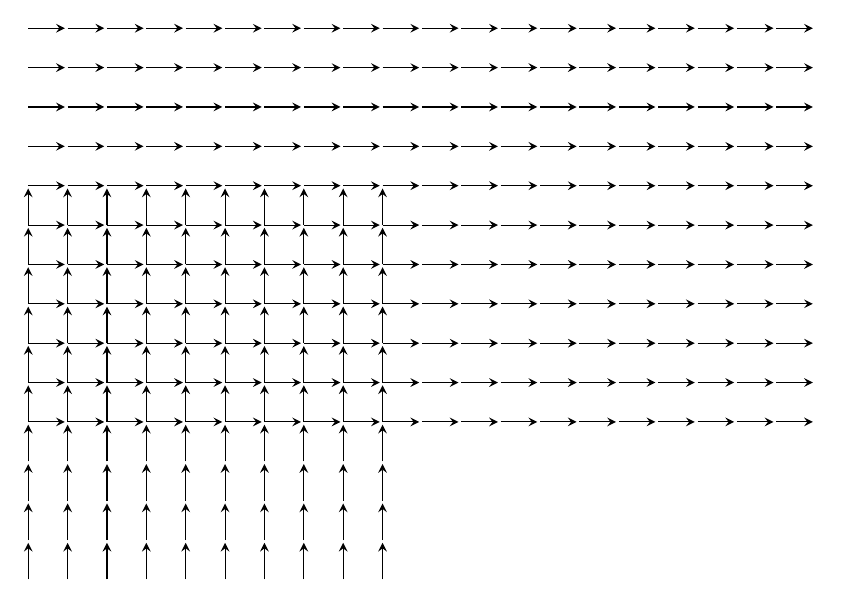
\begin{tikzpicture}[x=0.5cm,y=0.5cm,>=stealth,shorten >=1pt]
\foreach \x in {1,...,10}{
    \foreach \y in {1,...,10}{
	\draw[->] (\x,\y) -- (\x,\y+1);
    }
}
\foreach \x in {1,...,20}{
    \foreach \y in {5,...,15}{
	\draw[->] (\x,\y) -- (\x+1,\y);
    }
}
\end{tikzpicture}
\end{center}
\caption{The relation from \autoref{ex:closure4}}
\label{f:closure4}
\end{figure}
\begin{example}
\label{ex:closure4}
Consider the relation in example {\tt closure4} that comes with
the Omega calculator~\shortcite{Omega_calc}, $R = R_1 \cup R_2$,
with
$$
\begin{aligned}
R_1 & = \{\, (x,y) \to (x,y+1) \mid 1 \le x,y \le 10 \,\}
\\
R_2 & = \{\, (x,y) \to (x+1,y) \mid 1 \le x \le 20 \wedge 5 \le y \le 15 \,\}
.
\end{aligned}
$$
This relation is shown graphically in \autoref{f:closure4}.
We have
$$
\begin{aligned}
R_1 \circ R_2 &=
\{\, (x,y) \to (x+1,y+1) \mid 1 \le x \le 9 \wedge 5 \le y \le 10 \,\}
\\
R_2 \circ R_1 &=
\{\, (x,y) \to (x+1,y+1) \mid 1 \le x \le 10 \wedge 4 \le y \le 10 \,\}
.
\end{aligned}
$$
Clearly, $R_1 \circ R_2 \subseteq R_2 \circ R_1$ and so
$$
\left(
R_1 \cup R_2
\right)^+
=
\left(R_2^+ \circ R_1^+\right)
\cup R_1^+
\cup R_2^+
.
$$
\end{example}

\begin{figure}
\newcounter{n}
\newcounter{t1}
\newcounter{t2}
\newcounter{t3}
\newcounter{t4}
\begin{center}
\begin{tikzpicture}[>=stealth,shorten >=1pt]
\setcounter{n}{7}
\foreach \i in {1,...,\value{n}}{
    \foreach \j in {1,...,\value{n}}{
	\setcounter{t1}{2 * \j - 4 - \i + 1}
	\setcounter{t2}{\value{n} - 3 - \i + 1}
	\setcounter{t3}{2 * \i - 1 - \j + 1}
	\setcounter{t4}{\value{n} - \j + 1}
	\ifnum\value{t1}>0\ifnum\value{t2}>0
	\ifnum\value{t3}>0\ifnum\value{t4}>0
	    \draw[thick,->] (\i,\j) to[out=20] (\i+3,\j);
	\fi\fi\fi\fi
	\setcounter{t1}{2 * \j - 1 - \i + 1}
	\setcounter{t2}{\value{n} - \i + 1}
	\setcounter{t3}{2 * \i - 4 - \j + 1}
	\setcounter{t4}{\value{n} - 3 - \j + 1}
	\ifnum\value{t1}>0\ifnum\value{t2}>0
	\ifnum\value{t3}>0\ifnum\value{t4}>0
	    \draw[thick,->] (\i,\j) to[in=-20,out=20] (\i,\j+3);
	\fi\fi\fi\fi
	\setcounter{t1}{2 * \j - 1 - \i + 1}
	\setcounter{t2}{\value{n} - 1 - \i + 1}
	\setcounter{t3}{2 * \i - 1 - \j + 1}
	\setcounter{t4}{\value{n} - 1 - \j + 1}
	\ifnum\value{t1}>0\ifnum\value{t2}>0
	\ifnum\value{t3}>0\ifnum\value{t4}>0
	    \draw[thick,->] (\i,\j) to (\i+1,\j+1);
	\fi\fi\fi\fi
    }
}
\end{tikzpicture}
\end{center}
\caption{The relation from \autoref{ex:decomposition}}
\label{f:decomposition}
\end{figure}
\begin{example}
\label{ex:decomposition}
Consider the relation on the right of \shortciteN[Figure~2]{Beletska2009},
reproduced in \autoref{f:decomposition}.
The relation can be described as $R = R_1 \cup R_2 \cup R_3$,
with
$$
\begin{aligned}
R_1 &= n \mapsto \{\, (i,j) \to (i+3,j) \mid
i \le 2 j - 4 \wedge
i \le n - 3 \wedge
j \le 2 i - 1 \wedge
j \le n \,\}
\\
R_2 &= n \mapsto \{\, (i,j) \to (i,j+3) \mid
i \le 2 j - 1 \wedge
i \le n \wedge
j \le 2 i - 4 \wedge
j \le n - 3 \,\}
\\
R_3 &= n \mapsto \{\, (i,j) \to (i+1,j+1) \mid
i \le 2 j - 1 \wedge
i \le n - 1 \wedge
j \le 2 i - 1 \wedge
j \le n - 1\,\}
.
\end{aligned}
$$
The figure shows this relation for $n = 7$.
Both
$R_3 \circ R_1 \subseteq R_1 \circ R_3$
and
$R_3 \circ R_2 \subseteq R_2 \circ R_3$,
which the reader can verify using the {\tt iscc} calculator:
\begin{verbatim}
R1 := [n] -> { [i,j] -> [i+3,j] : i <= 2 j - 4 and i <= n - 3 and
                                  j <= 2 i - 1 and j <= n };
R2 := [n] -> { [i,j] -> [i,j+3] : i <= 2 j - 1 and i <= n and
                                  j <= 2 i - 4 and j <= n - 3 };
R3 := [n] -> { [i,j] -> [i+1,j+1] : i <= 2 j - 1 and i <= n - 1 and
                                    j <= 2 i - 1 and j <= n - 1 };
(R1 . R3) - (R3 . R1);
(R2 . R3) - (R3 . R2);
\end{verbatim}
$R_3$ can therefore be moved forward in any path.
For the other two basic relations, we have both
$R_2 \circ R_1 \not\subseteq R_1 \circ R_2$
and
$R_1 \circ R_2 \not\subseteq R_2 \circ R_1$
and so $R_1$ and $R_2$ form a strongly connected component.
By computing the power of $R_3$ and $R_1 \cup R_2$ separately
and composing the results, the power of $R$ can be computed exactly
using \eqref{eq:transitive:singleton}.
As explained by \shortciteN{Beletska2009}, applying the same formula
to $R$ directly, without a decomposition, would result in
an overapproximation of the power.
\end{example}

\subsection{Partitioning the domains and ranges of $R$}

The algorithm of \autoref{s:power} assumes that the input relation $R$
can be treated as a union of translations.
This is a reasonable assumption if $R$ maps elements of a given
abstract domain to the same domain.
However, if $R$ is a union of relations that map between different
domains, then this assumption no longer holds.
In particular, when an entire dependence graph is encoded
in a single relation, as is done by, e.g.,
\shortciteN[Section~6.1]{Barthou2000MSE}, then it does not make
sense to look at differences between iterations of different domains.
Now, arguably, a modified Floyd-Warshall algorithm should
be applied to the dependence graph, as advocated by
\shortciteN{Kelly1996closure}, with the transitive closure operation
only being applied to relations from a given domain to itself.
However, it is also possible to detect disjoint domains and ranges
and to apply Floyd-Warshall internally.

\linesnumbered
\begin{algorithm}
\caption{The modified Floyd-Warshall algorithm of
\protect\shortciteN{Kelly1996closure}}
\label{a:Floyd}
\SetKwInput{Input}{Input}
\SetKwInput{Output}{Output}
\Input{Relations $R_{pq}$, $0 \le p, q < n$}
\Output{Updated relations $R_{pq}$ such that each relation
$R_{pq}$ contains all indirect paths from $p$ to $q$ in the input graph}
%
\BlankLine
\SetVline
\dontprintsemicolon
%
\For{$r \in [0, n-1]$}{
    $R_{rr} \coloneqq R_{rr}^+$ \nllabel{l:Floyd:closure}\;
    \For{$p \in [0, n-1]$}{
	\For{$q \in [0, n-1]$}{
	    \If{$p \ne r$ or $q \ne r$}{
		$R_{pq} \coloneqq R_{pq} \cup \left(R_{rq} \circ R_{pr}\right)
			     \cup \left(R_{rq} \circ R_{rr} \circ R_{pr}\right)$
	     \nllabel{l:Floyd:update}
	     }
	}
    }
}
\end{algorithm}

Let the input relation $R$ be a union of $m$ basic relations $R_i$.
Let $D_{2i}$ be the domains of $R_i$ and $D_{2i+1}$ the ranges of $R_i$.
The first step is to group overlapping $D_j$ until a partition is
obtained.  If the resulting partition consists of a single part,
then we continue with the algorithm of \autoref{s:power}.
Otherwise, we apply Floyd-Warshall on the graph with as vertices
the parts of the partition and as edges the $R_i$ attached to
the appropriate pairs of vertices.
In particular, let there be $n$ parts $P_k$ in the partition.
We construct $n^2$ relations
$$
R_{pq} \coloneqq \bigcup_{i \text{ s.t. } \domain R_i \subseteq P_p \wedge
				 \range R_i \subseteq P_q} R_i
,
$$
apply \autoref{a:Floyd} and return the union of all resulting
$R_{pq}$ as the transitive closure of $R$.
Each iteration of the $r$-loop in \autoref{a:Floyd} updates
all relations $R_{pq}$ to include paths that go from $p$ to $r$,
possibly stay there for a while, and then go from $r$ to $q$.
Note that paths that ``stay in $r$'' include all paths that
pass through earlier vertices since $R_{rr}$ itself has been updated
accordingly in previous iterations of the outer loop.
In principle, it would be sufficient to use the $R_{pr}$
and $R_{rq}$ computed in the previous iteration of the
$r$-loop in Line~\ref{l:Floyd:update}.
However, from an implementation perspective, it is easier
to allow either or both of these to have been updated
in the same iteration of the $r$-loop.
This may result in duplicate paths, but these can usually
be removed by coalescing (\autoref{s:coalescing}) the result of the union
in Line~\ref{l:Floyd:update}, which should be done in any case.
The transitive closure in Line~\ref{l:Floyd:closure}
is performed using a recursive call.  This recursive call
includes the partitioning step, but the resulting partition will
usually be a singleton.
The result of the recursive call will either be exact or an
overapproximation.  The final result of Floyd-Warshall is therefore
also exact or an overapproximation.

\begin{figure}
\begin{center}
\begin{tikzpicture}[x=1cm,y=1cm,>=stealth,shorten >=3pt]
\foreach \x/\y in {0/0,1/1,3/2} {
    \fill (\x,\y) circle (2pt);
}
\foreach \x/\y in {0/1,2/2,3/3} {
    \draw (\x,\y) circle (2pt);
}
\draw[->] (0,0) -- (0,1);
\draw[->] (0,1) -- (1,1);
\draw[->] (2,2) -- (3,2);
\draw[->] (3,2) -- (3,3);
\draw[->,dashed] (2,2) -- (3,3);
\draw[->,dotted] (0,0) -- (1,1);
\end{tikzpicture}
\end{center}
\caption{The relation (solid arrows) on the right of Figure~1 of
\protect\shortciteN{Beletska2009} and its transitive closure}
\label{f:COCOA:1}
\end{figure}
\begin{example}
Consider the relation on the right of Figure~1 of
\shortciteN{Beletska2009},
reproduced in \autoref{f:COCOA:1}.
This relation can be described as
$$
\begin{aligned}
\{\, (x, y) \to (x_2, y_2) \mid {} & (3y = 2x \wedge x_2 = x \wedge 3y_2 = 3 + 2x \wedge x \ge 0 \wedge x \le 3) \vee {} \\
& (x_2 = 1 + x \wedge y_2 = y \wedge x \ge 0 \wedge 3y \ge 2 + 2x \wedge x \le 2 \wedge 3y \le 3 + 2x) \,\}
.
\end{aligned}
$$
Note that the domain of the upward relation overlaps with the range
of the rightward relation and vice versa, but that the domain
of neither relation overlaps with its own range or the domain of
the other relation.
The domains and ranges can therefore be partitioned into two parts,
$P_0$ and $P_1$, shown as the white and black dots in \autoref{f:COCOA:1},
respectively.
Initially, we have
$$
\begin{aligned}
R_{00} & = \emptyset
\\
R_{01} & = 
\{\, (x, y) \to (x+1, y) \mid 
(x \ge 0 \wedge 3y \ge 2 + 2x \wedge x \le 2 \wedge 3y \le 3 + 2x) \,\}
\\
R_{10} & =
\{\, (x, y) \to (x_2, y_2) \mid (3y = 2x \wedge x_2 = x \wedge 3y_2 = 3 + 2x \wedge x \ge 0 \wedge x \le 3) \,\}
\\
R_{11} & = \emptyset
.
\end{aligned}
$$
In the first iteration, $R_{00}$ remains the same ($\emptyset^+ = \emptyset$).
$R_{01}$ and $R_{10}$ are therefore also unaffected, but
$R_{11}$ is updated to include $R_{01} \circ R_{10}$, i.e.,
the dashed arrow in the figure.
This new $R_{11}$ is obviously transitively closed, so it is not
changed in the second iteration and it does not have an effect
on $R_{01}$ and $R_{10}$.  However, $R_{00}$ is updated to
include $R_{10} \circ R_{01}$, i.e., the dotted arrow in the figure.
The transitive closure of the original relation is then equal to
$R_{00} \cup R_{01} \cup R_{10} \cup R_{11}$.
\end{example}

\subsection{An {\tt Omega}-like implementation}

While the main algorithm of \shortciteN{Kelly1996closure} is
designed to compute and underapproximation of the transitive closure,
the authors mention that they could also compute overapproximations.
In this section, we describe our implementation of an algorithm
that is based on their ideas.
Note that the {\tt Omega} library computes underapproximations
\shortcite[Section 6.4]{Omega_lib}.

The main tool is Equation~(2) of \shortciteN{Kelly1996closure}.
The input relation $R$ is first overapproximated by a ``d-form'' relation
$$
\{\, \vec i \to \vec j \mid \exists \vec \alpha :
\vec L \le \vec j - \vec i \le \vec U
\wedge
(\forall p : j_p - i_p = M_p \alpha_p)
\,\}
,
$$
where $p$ ranges over the dimensions and $\vec L$, $\vec U$ and
$\vec M$ are constant integer vectors.  The elements of $\vec U$
may be $\infty$, meaning that there is no upper bound corresponding
to that element, and similarly for $\vec L$.
Such an overapproximation can be obtained by computing strides,
lower and upper bounds on the difference set $\Delta \, R$.
The transitive closure of such a ``d-form'' relation is
\begin{equation}
\label{eq:omega}
\{\, \vec i \to \vec j \mid \exists \vec \alpha, k :
k \ge 1 \wedge
k \, \vec L \le \vec j - \vec i \le k \, \vec U
\wedge
(\forall p : j_p - i_p = M_p \alpha_p)
\,\}
.
\end{equation}
The domain and range of this transitive closure are then
intersected with those of the input relation.
This is a special case of the algorithm in \autoref{s:power}.

In their algorithm for computing lower bounds, the authors
use the above algorithm as a substep on the disjuncts in the relation.
At the end, they say
\begin{quote}
If an upper bound is required, it can be calculated in a manner
similar to that of a single conjunct [sic] relation.
\end{quote}
Presumably, the authors mean that a ``d-form'' approximation
of the whole input relation should be used.
However, the accuracy can be improved by also using the following
idea from the same paper.  If $R$ is a union of $m$ basic maps,
$$
R = \bigcup_i R_i
,
$$
and if we can find an $R_i$ such that for all other $R_j$ we have
that
$$
R_i^* \circ R_j \circ R_i^*
$$
can be represented as a single basic map, i.e., without a union,
then we can compute $R^+$ as
$$
R^+ = R_i^+ \cup
\left(
\bigcup_{j \ne i}
R_i^* \circ R_j \circ R_i^*
\right)^+
,
$$
reducing the number of disjuncts in the argument of the transitive
closure by one.
An overapproximation of $R_i^*$ can be obtained by
allowing the value zero for $k$ in \eqref{eq:omega},
i.e., by computing
$$
\{\, \vec i \to \vec j \mid \exists \vec \alpha, k :
k \ge 0 \wedge
k \, \vec L \le \vec j - \vec i \le k \, \vec U
\wedge
(\forall p : j_p - i_p = M_p \alpha_p)
\,\}
.
$$
However, when we intersect domain and range of this relation
with those of the input relation, then the result only contains
the identity mapping on the intersection of domain and range.
\shortciteN{Kelly1996closure} propose to intersect domain
and range with then {\em union} of domain and range of the input
relation instead and call the result $R_i^?$.
Now, this union of domain and range of $R_i$ may not contain
the domains and ranges of the whole of $R$.
We can therefore not always replace
$R_i^* \circ R_j \circ R_i^*$ by
$R_i^? \circ R_j \circ R_i^?$.
\shortciteN{Kelly1996closure} propose to check the following
conditions to decide whether this replacement is justified:
$R_i^? - R_i^+$ is not a union and for each $j \ne i$
the condition
$$
\left(R_i^? - R_i^+\right)
\circ
R_j
\circ
\left(R_i^? - R_i^+\right)
=
R_j
$$
holds.
